\chapter{Towards Learning in Linear Models}

\section{Advanced Problem Formulations (Slides)}

The below are a list of major subject areas in NeurIPS \footnote[1][]{As of 2024, when the slides were created.}:
\begin{itemize}[noitemsep]
    \item Supervised, Unsupervised or Semi-Supervised Learning:
    \begin{itemize}[noitemsep]
        \item Few-shot Learning
        \item Transfer Learning
    \end{itemize}
    \item Unsupervised Learning:
    \begin{itemize}[noitemsep]
        \item Density Estimation
        \item Clustering
        \item Dimensionality Reduction
    \end{itemize}
\end{itemize}


\subsection{Few-shot Learning}

In supervised learning, let us define the notation:

\noindent Let our feature vector (which is our input space) be defined by
\begin{equation}
    x \in \R^n
\end{equation}

\noindent Let our output labels be defined by
\begin{equation}
    y \in \R^m
\end{equation}

\noindent  Assume our dataset is i.i.d distributed and  $K >> n$, it is defined as 
\begin{equation}
    \mathcal{D} = \{(x^{(i)}, y^{(i)})\}_{i=1}^K 
\end{equation}

Our learning objective is to find the minimum error from our loss function $\mathcal{L}$.
\begin{equation}
    \min_\theta \left[ \mathcal{L}(f^\theta(x),y) \right]
\end{equation}

In the case of \textbf{few-shot learning}, a technique in ML where a model learns to perform a task proficiently with only a limited amount of training data. We do not have the luxury of $K \gg n$ and so our model must learn to generalise well, quickly. 


\begin{itemize}[noitemsep]
    \item When $K = n$:
    \begin{itemize}[noitemsep]
        \item \textbf{n-shot learning}: Trains with $n$ examples per class.
        \item Example: With $n=3$, learn to recognise animals like cats, dogs, and birds from three images each.
    \end{itemize}
    \item When $K = 0$:
    \begin{itemize}[noitemsep]
        \item \textbf{zero-shot learning}:\footnote[][]{Very popular with Large Language Models (LLMs) and also known as zero-shot prompting in this case.} Infers classes with no examples, using descriptions.
        \item Example: Identify an animal as a mammal based on descriptions of mammals being warm-blooded with hair.
    \end{itemize}
    \item When $K = nc$:
    \begin{itemize}[noitemsep]
        \item \textbf{n-way c-shot learning}: Trains with $c$ examples from each of $n$ classes.
        \item Example: In a 5-way 2-shot scenario, classify fruits like apples, oranges, bananas, grapes, pineapples from two images each.
    \end{itemize}
\end{itemize}


\subsection{Transfer Learning}

Transfer learning is a machine learning technique where a model trained on one task is re-purposed on a second related task. Let us define two datasets, $\mathcal{D}$ and $\mathcal{D}'$:

\begin{align}
    \mathcal{D} &= \{(x^{(i)}, y^{(i)})\}_{i=1}^N \quad \text{where } x^{(i)} \in \mathbb{R}^n, y^{(i)} \in \mathbb{R}^d \\
    \mathcal{D}' &= \{(x'^{(i)}, y'^{(i)})\}_{i=1}^{N'} \quad \text{where } x'^{(i)} \in \mathbb{R}^n, y'^{(i)} \in \mathbb{R}^d
\end{align}

We then define the functions used in transfer learning :\footnote[][]{Bear with the difference in notation here: the notes use $\phi$ to represent the feature extractor instead of $g$.}
\begin{align}
    g^\omega &: \mathbb{R}^n \rightarrow \mathbb{R}^l \\
    h^\kappa &: \mathbb{R}^l \rightarrow \mathbb{R}^d \\ 
    f^\theta &: \mathbb{R}^l \rightarrow \mathbb{R}^m
\end{align}

The function $g^\omega$ represents a feature extractor that maps input features from $\mathbb{R}^n$ to a latent space $\mathbb{R}^l$. The function $h^\kappa$ is a task-specific classifier or regressor for the old task, mapping the latent features to outputs in $\mathbb{R}^d$. The function $f^\theta$ is a classifier or regressor for the new task, also mapping the latent features to outputs in $\mathbb{R}^m$. \bigskip

The learning process in transfer learning typically involves two main steps:

\begin{enumerate}
    \item Pre-training on the old dataset $\mathcal{D}$:
   \begin{equation}
   \min_{\omega, \kappa} \mathbb{E}_{\mathcal{D}}[L(y, h^\kappa(g^\omega(x)))]
   \end{equation}
   This step involves optimising the parameters $\omega$ and $\kappa$ to minimise the expected loss $L$ on the old dataset $\mathcal{D}$, effectively training the feature extractor $g^\omega$ and the old task classifier $h^\kappa$.

    \item Fine-tuning on the new dataset $\mathcal{D}'$:
   \begin{equation}
   \min_{\omega, \theta} \mathbb{E}_{\mathcal{D}'}[L(y', f^\theta(g^\omega(x')))]
   \end{equation}
   In this step, the feature extractor $g^\omega$ is further optimised along with the new task classifier $f^\theta$ to minimise the loss on the new dataset $\mathcal{D}'$. The parameters $\omega$ are fine-tuned to adapt to the new task, leveraging the feature extraction capabilities learned from the old task.

\end{enumerate}

\subsection{Density Estimation, Clustering and Dimensionality Reduction}

Assume we have an unsupervised learning setup, with $x \in \R^n$ and our dataset $\mathcal{D} = \{ x_1, x_2, \ldots, x_K \}$ where data is i.i.d and  $K \gg n$.

Notes:
\begin{enumerate}
    \item  \textbf{Density Estimation} is to estimate the probability density function (pdf) of the data distribution. 
    \item  \textbf{Clustering} is to find a way to group data points as clusters. We typically first estimate how many clusters exists, then try to fit assign points to the clusters.
    \item \textbf{Dimensionality Reduction} involves finding latent factors and/or associations in the data. Even though though the spacec of the data is large, the effective dimensionality of the problem is small. For example, we can visualise the MNIST dataset of handdrawn digits from 1-10 in a 2D space with t-Distributed Stochastic Neighbor Embedding (t-SNE) in Figure \ref{fig:mnist-tsne}.

\begin{figure}[h]
    \centering
    \begin{subfigure}[b]{0.45\linewidth}
        \centering
        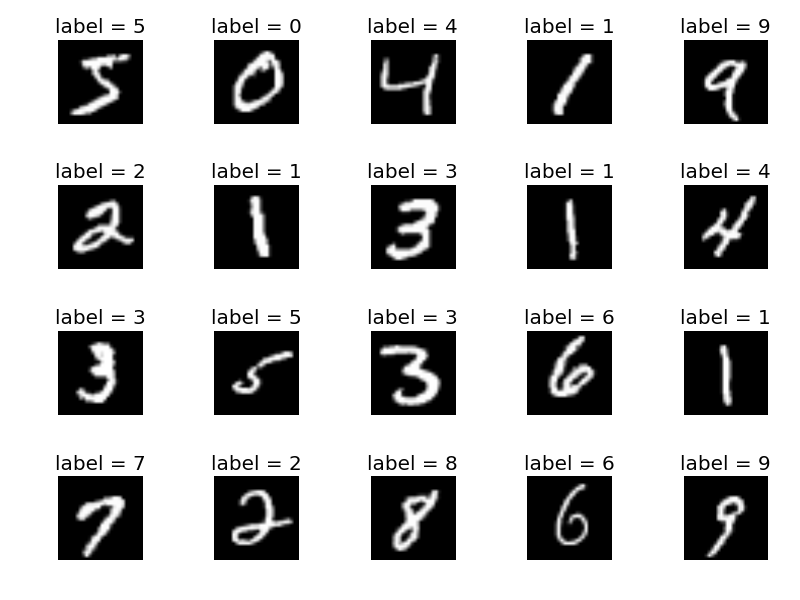
\includegraphics[width=\linewidth]{img/2_mnist.png}
        \caption{MNIST dataset}
    \end{subfigure}
    \hfill % optional; add some horizontal spacing
    \begin{subfigure}[b]{0.45\linewidth}
        \centering
        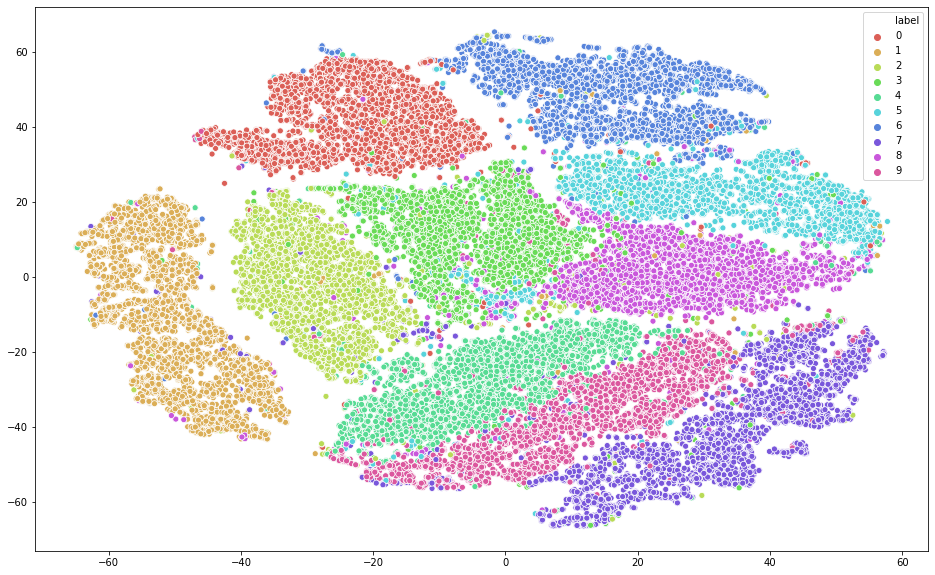
\includegraphics[width=\linewidth]{img/2_mnist-tsne.png}
        \caption{t-SNE visualisation on MNIST dataset}
        \label{fig:mnist-tsne}
    \end{subfigure}
    \caption{{\footnotesize MNIST dataset (dimension 10) and its corresponding t-SNE visualisation}}
    \label{fig:mnist-tsne}
\end{figure}




\end{enumerate}


\section{Supervised Learning}
Supervised learning assumes that we have access to input-output pairs of datapoints, $(\bm{x}, \bm{y})$, with $\bm{x} \in \mathbb{R}^n$ and $\bm{y} \in \mathbb{R}^m$, forming our dataset\sidenote{The slides replaced $K$ with $N$. Notation!} $\{(\bm{x}^{(i)}, \bm{y}^{(i)})\}_{i=1}^N$. 


\section{Linear Regression Model}
Assuming a domain of $\mathbb{R}^n$ and a one-dimensional co-domain, we can write our model as $f(\bm{x}) = \bm{x}^\top \bm{\theta}$. Thus we have:




\[
\hat{y}^{(i)} = \bm{x}^{(i)\top} \bm{\theta}
\]

The goal of learning is to find $\bm{\theta}$ such that $\hat{y}^{(i)} \approx y^{(i)}$. \marginnote{You may recall linear models written as affine transformations: $y = mx + b$, where $b$ is the bias or constant term – this makes the model affine and not linear. Linear models refers to the relationship between model parameters and predictions via a linear transformation.
}



\defb{Linear Transformation}{
A linear transformation between two vector spaces $V$ and $W$ is a map 

$$T : V \rightarrow W$$

such that:

\begin{itemize}
    \item $T(v_1 + v_2) = T(v_1) + T(v_2) \quad \forall v_1, v_2 \in V$
    \item $T(\alpha v) = \alpha T(v) \quad \forall v \in V \text{ and scalar }\alpha $
\end{itemize}

}

\marginnote[-70pt]{
    \defsb{Affine Transformations}{
        Affine transformations are more general than linear transformations, because they include not only scaling and rotation, but also translations.
    }
}


Now we are faced with something interesting: $T(\mb{0}) = \mb{0}$. According to our affine transformation $f(x) = mx+b $ where $m,b \in \mathbb{R}$, we have $f(0x) = b \neq 0f(x)$, which doesn't allow us to have a bias term $b$. This is easily fixed with a straightforward modification to capture the affine transformation $f(x) = mx + b$: we just add a feature to the input vector $x$ that is always equal to 1, then the corresponding weight for this feature becomes the bias. Introduce:

\begin{equation}
    \phi(x) : \mathbf{R} \Rightarrow \mathbf{R}^2 \quad \text{such that } \phi(x) = \begin{bmatrix} 1 \\ x \end{bmatrix} 
\end{equation}

\noindent We then need parameter vector $\theta = \begin{bmatrix} b \\ m \end{bmatrix}$. 

\noindent We then have the model 
\begin{equation}
    \hat{y} = \phi(x)^\top \theta \Rightarrow \begin{bmatrix} 1 & x \end{bmatrix}  \begin{bmatrix} b \\ m \end{bmatrix} = b + mx
\end{equation}

\section{Basis Expansion}
As seen in the previous section, a model that was once restricted to lines through the origin ahs been expanded to fit the affine transformation with the aid of Basis Expansion. We can also more generally utilise it to model non-linear relationships.

\bigskip

The key idea of basis expansion is to expand a one-dimensional feature into many dimensions, and use non-linear functions to increase the expressiveness of the model.

\subsection{Example Polynomial Basis Expansion}
A one dimensional domain $x \in \mathbb{R}$ and a one dimensional co-domain $y \in \mathbb{R}$ is assumed. Our model is $\hat{y} = \phi(x)^\top \theta$. \bigskip


We choose the basis:

\begin{equation}
    \phi(x) = \begin{bmatrix} 1 \\ x \\ x^2 \end{bmatrix} \quad \phi(x) : \R^1 \rightarrow \R^3
\end{equation}

and weights:

\begin{equation}
    \theta \in \mathbb{R}^3
\end{equation}

We finally have the fully expanded function\marginnote{We use the dot product instead of transposing, for clarity of notation.}:

\begin{equation}
    \hat{y} = \begin{bmatrix} 1 \\ x \\ x^2 \end{bmatrix} \cdot \begin{bmatrix} \theta_0 \\ \theta_1 \\ \theta_2 \end{bmatrix} = \theta_0 + \theta_1 x + \theta_2 x^2
\end{equation}

This example model is a quadratic polynomial. 

\subsection{Another Example Polynomial Basis Expansion}
Again, given our model is $\hat{y} = \phi(\mb{x})^\top \theta$ where $y \in \R $ and $\mb{x} \in \R^2$. We can use the basis

\begin{equation} 
    \phi(\mb{x}) \Rightarrow \phi\left(\begin{bmatrix} x_1 \\ x_2 \end{bmatrix}\right) = \begin{bmatrix} 1 \\ x_1 \\ x_2 \\ x_1x_2 \\ x_1^2 \\ x_2^2 \end{bmatrix} \quad \phi(x) : \mbb{R}^2 \rightarrow \mbb{R}^6
\end{equation}

and with a new set of corresponding weights, we have:

\begin{equation}
    \hat{y} = \begin{bmatrix} 1 \\ x_1 \\ x_2 \\ x_1x_2 \\ x_1^2 \\ x_2^2 \end{bmatrix} \cdot  \begin{bmatrix} \theta_0 \\ \theta_1 \\ \theta_2 \\ \theta_3 \\ \theta_4 \\ \theta_5 \end{bmatrix} = \theta_0 + \theta_1 x_1 + \theta_2 x_2 + \theta_3 x_1x_2 + \theta_4 x_1^2 + \theta_5 x_2^2 \quad \theta \in \mathbb{R}^6
\end{equation}

\section{Radial Basis Function Kernel}

Polynomial basis expansion is just a single flabour of basis expansion. Another widely-used form of basis is the kernel basis expansion. One popular example is the radial basis function kernel (RBF kernel), which is a generalisation of the polynomial basis expansion. \bigskip

It takes in a fixed parameter $\gamma > 0$, defined as 

\begin{equation}
    \kappa(x, x') = \exp(-\gamma ||x - x'||^2)
\end{equation}

where $||x - x'||^2$ is the squared Euclidean distance (or more appropriately, the $L_2$ Norm) between $x$ and $x'$. In practice, one picks fixed centres $x$ and the basis expansion computes the expanded feature set w.r.t the distance to these centres.\sidenote[][-130pt]{There is more nuance to this: you may have noticed that kernel functions take in two points, unlike the polynomial basis expansion $\phi$ taking in a single point. This is because for each of the $n$ points, we compute pairwise similarities with a point's other points, and then construct a feature vector for each point, where each point $x$ is transformed into a $n$-dimensional feature vector where each dimension represents the similarity between $x$ and one of the $n$ points.  \bigskip

For example, given a dataset with three points $x_1, x_2, x_3$, and a radial basis function $\kappa(x, x')$, the RBF kernel matrix might look like this:

\begin{equation*}
    K = \begin{bmatrix} \kappa(x_1, x_1) & \kappa(x_1, x_2) & \kappa(x_1, x_3) \\ \kappa(x_2, x_1) & \kappa(x_2, x_2) & \kappa(x_2, x_3) \\ \kappa(x_3, x_1) & \kappa(x_3, x_2) & \kappa(x_3, x_3) \end{bmatrix}
\end{equation*}

\noindent where the feature vector for $x_1$ as an example would be 
\[\begin{bmatrix} \kappa(x_1, x_1) & \kappa(x_1, x_2) & \kappa(x_1, x_3) \end{bmatrix}\]

\noindent This is related to the use of the \href{https://medium.com/@zxr.nju/what-is-the-kernel-trick-why-is-it-important-98a98db0961d}{kernel trick.}

}

\bigskip

\begin{itemize}
    \item It is easy to see that the kernel basis expansion $\kappa(x, x')$ has a minimum value of 0. It takes a maximum value of 1 when $x = x'$ . 
    \item When two points $x$ and $x'$ are far apart, the kernel value is closer to 0, and when they are closer together, the kernel value is closer to 1. 

    \item It is quite akin to a simiarity score, and that a smaller value of $\gamma$ leads to larger similarity scores (see Figure \ref{fig:rbf_kernel}).
    
    \item It is also symmetric, $\kappa(x, x') = \kappa(x', x)$, and is always positive. 
\end{itemize}

\bigskip
\begin{figure}[h]
    \centering
    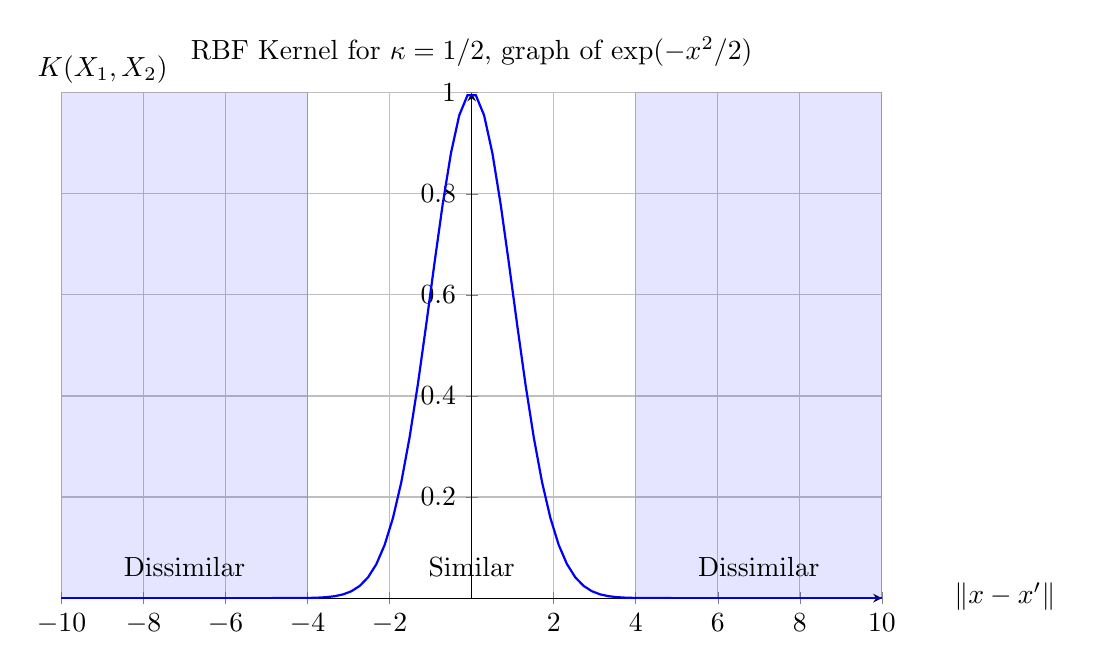
\begin{tikzpicture}
    \begin{axis}[
        width=12cm,
        height=8cm,
        xlabel={$\|x - x'\|$},
        ylabel={$K(X_1, X_2)$},
        grid=major,
        domain=-10:10,
        samples=100,
        xtick={-10,-8,...,10},
        ytick={0,0.2,...,1},
        enlargelimits=false,
        legend pos=outer north east,
        axis lines=middle,
        xlabel style={at={(axis description cs:1.15,0.05)},anchor=north},
        ylabel style={at={(axis description cs:0.05,1)},anchor=south},
        title={RBF Kernel for $\kappa = 1/2$, graph of $\exp(-x^2/2)$},
        ymin=0, ymax=1,
        xmin=-10, xmax=10
    ]
        \addplot [
            blue,
            thick,
            domain=-10:10,
        ]
        {exp(-x^2/2)};
        
        % Highlight regions
        \draw [fill=blue, opacity=0.1] (axis cs:-10,0) rectangle (axis cs:-4,1);
        \draw [fill=blue, opacity=0.1] (axis cs:4,0) rectangle (axis cs:10,1);
        
        % Add region labels
        \node at (axis cs:-7,0.1) [anchor=north] {Dissimilar};
        \node at (axis cs:7,0.1) [anchor=north] {Dissimilar};
        \node at (axis cs:0,0.1) [anchor=north] {Similar};
    
    \end{axis}
    \end{tikzpicture}
    \caption{RBF Kernel for $\kappa = 1/2$, graph of $\exp(-x^2/2)$. Areas of dissimilarity are noted when the kernel values are negligible.}
    \label{fig:rbf_kernel}
    \end{figure}
    
    The RBF kernel is actually a special case of the polynomial basis expansion, where 


\subsection{Example Radial Basis Function Kernel}
Given a one-dimensional domain and a one-dimensional co-domain, we have the model $\hat{y} = \phi(x)^\top \theta$.

\begin{equation}
    \phi(x) = \exp(-\gamma ||x - x'||^2) \quad \phi(x) : \mathbb{R}^1 \rightarrow \mathbb{R}^1
\end{equation}

and with a new set of corresponding weights, we have:

\begin{equation}
    \hat{y} = \exp(-\gamma ||x - x'||^2) \cdot \begin{bmatrix} \theta_0 \\ \theta_1 \end{bmatrix} = \theta_0 \exp(-\gamma ||x - x'||^2) + \theta_1
\end{equation}


\section{Linear Algebra}








